\documentclass[border=4pt]{standalone}
\usepackage[T1]{fontenc}
\usepackage{lmodern}
\usepackage{amsmath}
\usepackage{pgfplots}
\pgfplotsset{compat=1.18}
\usepgfplotslibrary{groupplots,fillbetween}
\usetikzlibrary{calc,arrows.meta}
% one colour per kind of method, the same in every figure (Okabe-Ito)
\definecolor{neur}{HTML}{D55E00}   % neurons chosen by attribution
\definecolor{dirc}{HTML}{009E73}   % directions from the weird-vs-normal contrast
\definecolor{read}{HTML}{0072B2}   % readout methods and interventions chosen from readouts
\definecolor{pers}{HTML}{CC79A7}   % Assistant Axis / persona
\definecolor{ctrl}{HTML}{8C8C8C}   % random controls
\definecolor{meas}{HTML}{E69F00}   % measured outcome
\definecolor{ink}{HTML}{222222}
\pgfplotsset{
  every axis/.append style={clip=false, font=\small, axis line style={black!55}, tick style={black!55}, tick align=outside,
    label style={font=\small}, tick label style={font=\footnotesize}, title style={font=\small, align=center}},
  grid style={black!9, line width=0.4pt},
  every axis legend/.append style={font=\footnotesize, draw=none, fill=none},
  ci/.style={/pgfplots/error bars/x dir=both, /pgfplots/error bars/x explicit, /pgfplots/error bars/error bar style={line width=0.8pt}, /pgfplots/error bars/error mark=none},
  yci/.style={/pgfplots/error bars/y dir=both, /pgfplots/error bars/y explicit, /pgfplots/error bars/error bar style={line width=0.8pt}, /pgfplots/error bars/error mark=none},
}

\usepackage{CJKutf8}
\usepackage{array}
\begin{document}
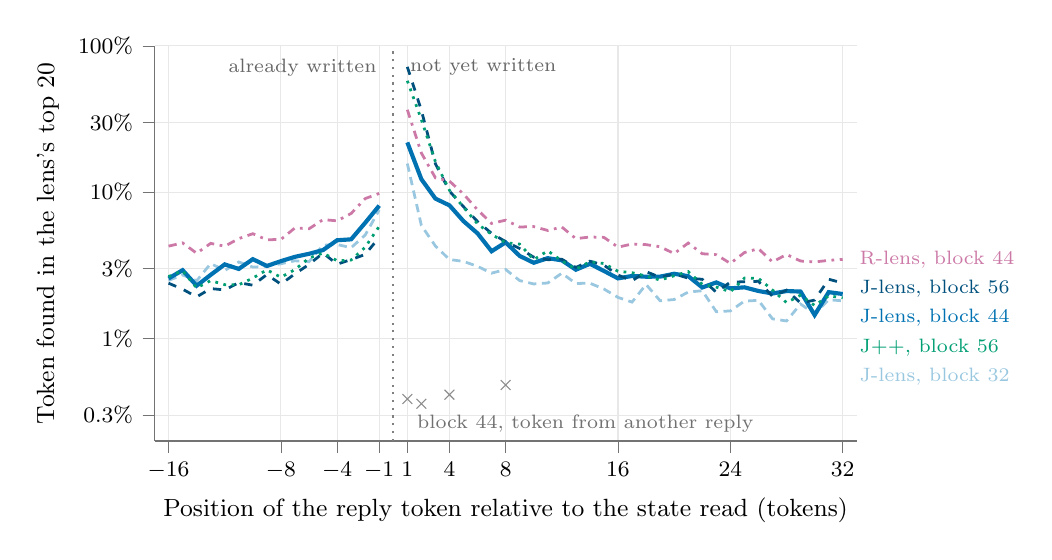
\begin{tikzpicture}
\begin{axis}[width=10.5cm, height=6.6cm, xmin=-17, xmax=33, xtick={-16,-8,-4,-1,1,4,8,16,24,32}, ymode=log, ymin=0.002, ymax=1, ytick={0.003,0.01,0.03,0.1,0.3,1}, yticklabels={0.3\%,1\%,3\%,10\%,30\%,100\%}, axis x line*=bottom, axis y line*=left, grid=major, xlabel={Position of the reply token relative to the state read (tokens)}, ylabel={Token found in the lens's top 20}]
\draw[black!50, dotted, line width=0.8pt] (axis cs:0,0.002) -- (axis cs:0,1);
\node[font=\scriptsize, black!60, anchor=north east] at (axis cs:-0.5,0.95) {already written};
\node[font=\scriptsize, black!60, anchor=north west] at (axis cs:0.5,0.95) {not yet written};
\addplot[read!40, line width=1.0pt, densely dashed] coordinates {(-16,0.02496) (-15,0.02725) (-14,0.02483) (-13,0.03256) (-12,0.02921) (-11,0.03338) (-10,0.03081) (-9,0.03109) (-8,0.03248) (-7,0.03401) (-6,0.03353) (-5,0.04342) (-4,0.04393) (-3,0.04179) (-2,0.05100) (-1,0.07567)};
\addplot[read!40, line width=1.0pt, densely dashed] coordinates {(1,0.15698) (2,0.05930) (3,0.04291) (4,0.03471) (5,0.03369) (6,0.03115) (7,0.02800) (8,0.02967) (9,0.02491) (10,0.02363) (11,0.02399) (12,0.02797) (13,0.02381) (14,0.02390) (15,0.02181) (16,0.01913) (17,0.01777) (18,0.02344) (19,0.01814) (20,0.01849) (21,0.02080) (22,0.02124) (23,0.01527) (24,0.01546) (25,0.01804) (26,0.01826) (27,0.01365) (28,0.01320) (29,0.01723) (30,0.01478) (31,0.01843) (32,0.01812)};
\addplot[read, line width=1.5pt] coordinates {(-16,0.02575) (-15,0.02935) (-14,0.02298) (-13,0.02726) (-12,0.03213) (-11,0.02993) (-10,0.03490) (-9,0.03136) (-8,0.03383) (-7,0.03620) (-6,0.03796) (-5,0.04026) (-4,0.04698) (-3,0.04766) (-2,0.06181) (-1,0.08097)};
\addplot[read, line width=1.5pt] coordinates {(1,0.21894) (2,0.12275) (3,0.09044) (4,0.08133) (5,0.06346) (6,0.05235) (7,0.03952) (8,0.04544) (9,0.03670) (10,0.03297) (11,0.03544) (12,0.03427) (13,0.02956) (14,0.03242) (15,0.02899) (16,0.02579) (17,0.02679) (18,0.02648) (19,0.02651) (20,0.02773) (21,0.02671) (22,0.02236) (23,0.02420) (24,0.02204) (25,0.02241) (26,0.02115) (27,0.02033) (28,0.02113) (29,0.02096) (30,0.01449) (31,0.02077) (32,0.02017)};
\addplot[read!70!black, line width=1.0pt, dashed] coordinates {(-16,0.02391) (-15,0.02175) (-14,0.01928) (-13,0.02197) (-12,0.02151) (-11,0.02411) (-10,0.02317) (-9,0.02737) (-8,0.02355) (-7,0.02770) (-6,0.03214) (-5,0.03842) (-4,0.03225) (-3,0.03466) (-2,0.03760) (-1,0.04917)};
\addplot[read!70!black, line width=1.0pt, dashed] coordinates {(1,0.71846) (2,0.36270) (3,0.15647) (4,0.10179) (5,0.07966) (6,0.06307) (7,0.05234) (8,0.04598) (9,0.04125) (10,0.03599) (11,0.03462) (12,0.03482) (13,0.03065) (14,0.03379) (15,0.03175) (16,0.02718) (17,0.02482) (18,0.02868) (19,0.02623) (20,0.02773) (21,0.02586) (22,0.02543) (23,0.02074) (24,0.02433) (25,0.02445) (26,0.02463) (27,0.01945) (28,0.02142) (29,0.01751) (30,0.01833) (31,0.02545) (32,0.02397)};
\addplot[dirc, line width=1.0pt, dotted] coordinates {(-16,0.02654) (-15,0.02909) (-14,0.02219) (-13,0.02488) (-12,0.02337) (-11,0.02331) (-10,0.02590) (-9,0.02950) (-8,0.02625) (-7,0.02962) (-6,0.03547) (-5,0.03842) (-4,0.03403) (-3,0.03440) (-2,0.04207) (-1,0.05850)};
\addplot[dirc, line width=1.0pt, dotted] coordinates {(1,0.57721) (2,0.31338) (3,0.16161) (4,0.10308) (5,0.07913) (6,0.06078) (7,0.05156) (8,0.04518) (9,0.04420) (10,0.03462) (11,0.03980) (12,0.03400) (13,0.02983) (14,0.03352) (15,0.03258) (16,0.02884) (17,0.02820) (18,0.02675) (19,0.02511) (20,0.02689) (21,0.02868) (22,0.02348) (23,0.02247) (24,0.02090) (25,0.02590) (26,0.02579) (27,0.02149) (28,0.01761) (29,0.01981) (30,0.01685) (31,0.01960) (32,0.01900)};
\addplot[pers, line width=1.0pt, dashdotted] coordinates {(-16,0.04283) (-15,0.04507) (-14,0.03830) (-13,0.04473) (-12,0.04275) (-11,0.04821) (-10,0.05207) (-9,0.04730) (-8,0.04763) (-7,0.05705) (-6,0.05625) (-5,0.06500) (-4,0.06374) (-3,0.07161) (-2,0.09048) (-1,0.09813)};
\addplot[pers, line width=1.0pt, dashdotted] coordinates {(1,0.36597) (2,0.18537) (3,0.12539) (4,0.11914) (5,0.09715) (6,0.07584) (7,0.06124) (8,0.06442) (9,0.05786) (10,0.05824) (11,0.05480) (12,0.05786) (13,0.04817) (14,0.04945) (15,0.04914) (16,0.04215) (17,0.04428) (18,0.04385) (19,0.04241) (20,0.03810) (21,0.04498) (22,0.03801) (23,0.03745) (24,0.03264) (25,0.03871) (26,0.04115) (27,0.03339) (28,0.03756) (29,0.03388) (30,0.03341) (31,0.03422) (32,0.03479)};
\node[font=\scriptsize, pers, anchor=west] at (axis cs:32.5,0.03479) {R-lens, block 44};
\node[font=\scriptsize, read!70!black, anchor=west] at (axis cs:32.5,0.02195) {J-lens, block 56};
\node[font=\scriptsize, read, anchor=west] at (axis cs:32.5,0.01385) {J-lens, block 44};
\node[font=\scriptsize, dirc, anchor=west] at (axis cs:32.5,0.00874) {J++, block 56};
\node[font=\scriptsize, read!40, anchor=west] at (axis cs:32.5,0.00551) {J-lens, block 32};
\addplot[ctrl, only marks, mark=x, mark size=2.5pt] coordinates {(1,0.00387) (2,0.00359) (4,0.00414) (8,0.00482)};
\node[font=\scriptsize, ctrl!80!black, anchor=north west] at (axis cs:1,0.00348) {block 44, token from another reply};
\end{axis}
\end{tikzpicture}
\end{document}
